\captionsetup[figure]{labelformat=empty,font=scriptsize,labelfont=scriptsize}
\begin{frame}{Application-specific Optimizations Don't Generalize}
  \pgfplotstableread[row sep=\\,col sep=&]{
    Frame Rate & Bandwidth (normalized) & Accuracy \\
    30 & 100 & 100 \\
    10 & 40 & 92 \\
     5 & 21 & 90 \\
     3 & 13 & 87 \\
     2 & 9 & 84 \\
  }\stationaryframerate
  \pgfplotstableread[row sep=\\,col sep=&]{
    Resolution & Bandwidth (normalized) & Accuracy \\
    1080p & 100 & 100 \\
    900p & 79 & 87 \\
    720p & 54 & 84 \\
    540p & 29 & 71 \\
    360p & 17 & 11 \\
  }\stationaryresolution

  \begin{columns}[c]
    \column{0.4\textwidth}
    \vspace{2em}
    \begin{figure}
      \centering
      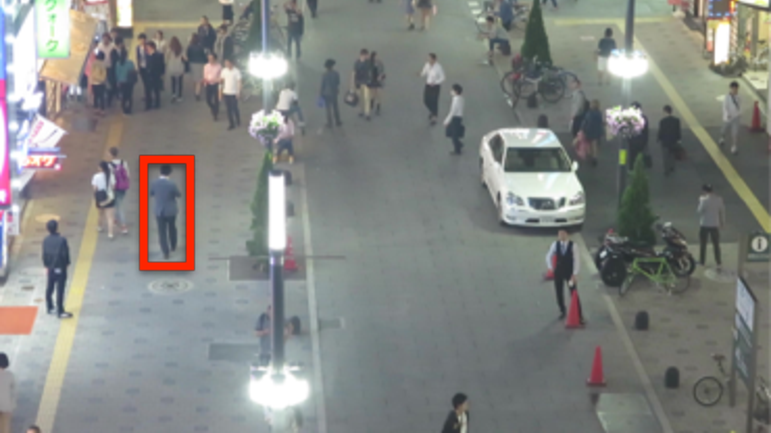
\includegraphics[width=\linewidth]{figures/mot-1.pdf}
      \caption{t=0s, small target in far-field views}
    \end{figure}
    \vspace{-1em}
    \begin{figure}
      \centering
      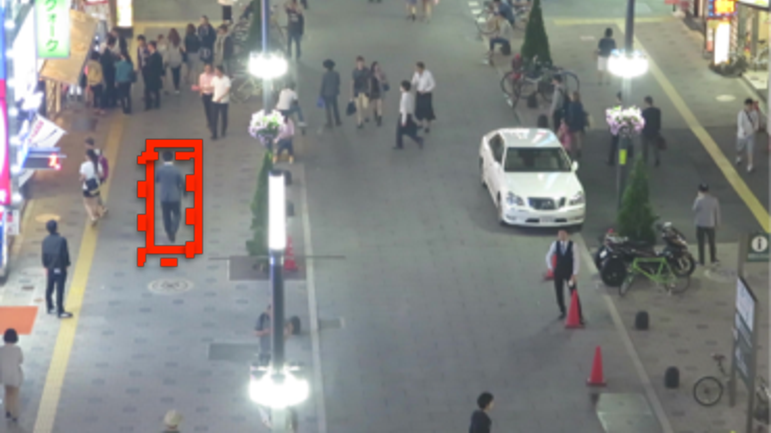
\includegraphics[width=\linewidth]{figures/mot-2.pdf}
      \caption{t=1s, small difference}
    \end{figure}

    \column{0.6\textwidth}
    \vspace{1.5em}

    \begin{tikzpicture}
      \tikzstyle{every node}=[font=\footnotesize]
      \begin{axis}[
        ybar,
        bar width               = .4cm,
        width                   = 1.1\textwidth,
        height                  = 0.4\textheight,
        legend style            = {at = {(0.5, 1.4)}, anchor = north,legend columns = -1},
        symbolic x coords       = {30, 10, 5, 3, 2},
        xtick                   = data,
        enlarge x limits        = 0.15,
        ymin                    = 0,
        ymax                    = 130,
        xlabel                  = {Frame Rate},
        nodes near coords,
        nodes near coords align = {vertical},
        ]
        \addplot table[x=Frame Rate,y=Bandwidth (normalized)]{\stationaryframerate};
        \addplot table[x=Frame Rate,y=Accuracy]{\stationaryframerate};
        \legend{Bandwidth (normalized), Accuracy}
      \end{axis}
    \end{tikzpicture}

    \vspace{1em}

    \begin{tikzpicture}
      \tikzstyle{every node}=[font=\footnotesize]
      \begin{axis}[
        ybar,
        bar width               = .4cm,
        width                   = 1.1\textwidth,
        height                  = 0.4\textheight,
        symbolic x coords       = {1080p, 900p, 720p, 540p, 360p},
        xtick                   = data,
        enlarge x limits        = 0.15,
        nodes near coords,
        nodes near coords align = {vertical},
        ymin                    = 0,
        ymax                    = 130,
        xlabel                  = {Resolution},
        ]
        \addplot table[x = Resolution, y = Bandwidth (normalized)]{\stationaryresolution};
        \addplot table[x = Resolution, y = Accuracy]{\stationaryresolution};
        \legend{}
      \end{axis}
    \end{tikzpicture}
  \end{columns}
\end{frame}


\begin{frame}{Application-specific Optimizations Don't Generalize}
  \captionsetup[figure]{labelformat=empty,font=scriptsize,labelfont=scriptsize}

  \pgfplotstableread[row sep=\\,col sep=&]{
    Frame Rate & Bandwidth (normalized) & Accuracy \\
    30 & 100 & 100 \\
    10 & 65 & 64 \\
    5 & 46 & 32 \\
    3 & 34 & 18 \\
    2 & 27 & 10 \\
  }\mobileframerate
  \pgfplotstableread[row sep=\\,col sep=&]{
    Resolution & Bandwidth (normalized) & Accuracy \\
    1080p & 100 & 100 \\
    900p & 69 & 99 \\
    720p & 49 & 97 \\
    540p & 33 & 93 \\
    360p & 22 & 87 \\
  }\mobileresolution

  \begin{columns}[c]
    \column{0.4\textwidth}
    \vspace{2em}
    \begin{figure}
      \centering
      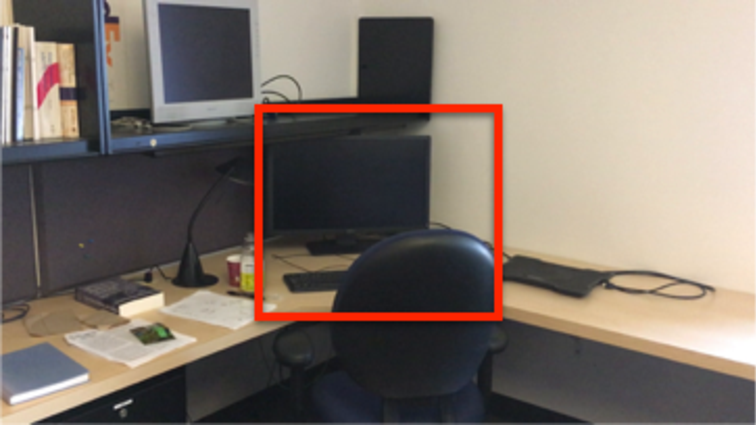
\includegraphics[width=\linewidth]{figures/darknet-1.pdf}
      \caption{t=0s, nearby and large targets}
    \end{figure}
    \vspace{-1em}
    \begin{figure}
      \centering
      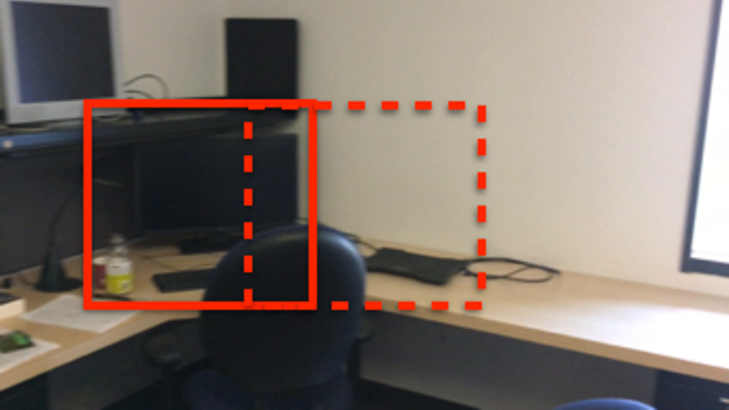
\includegraphics[width=\linewidth]{figures/darknet-2.pdf}
      \caption{t=1s, large difference}
    \end{figure}

    \column{0.6\textwidth}
    \vspace{1.5em}

    \begin{tikzpicture}
      \tikzstyle{every node}=[font=\footnotesize]
      \begin{axis}[
        ybar,
        bar width               = .4cm,
        width                   = 1.1\textwidth,
        height                  = 0.4\textheight,
        legend style            = {at = {(0.5, 1.4)}, anchor = north,legend columns = -1},
        symbolic x coords       = {30, 10, 5, 3, 2},
        xtick                   = data,
        enlarge x limits        = 0.15,
        ymin                    = 0,
        ymax                    = 130,
        xlabel                  = {Frame Rate},
        nodes near coords,
        nodes near coords align = {vertical},
        ]
        \addplot table[x=Frame Rate,y=Bandwidth (normalized)]{\mobileframerate};
        \addplot table[x=Frame Rate,y=Accuracy]{\mobileframerate};
        \legend{Bandwidth (normalized), Accuracy}
      \end{axis}
    \end{tikzpicture}

    \vspace{1em}

    \begin{tikzpicture}
      \tikzstyle{every node}=[font=\footnotesize]
      \begin{axis}[
        ybar,
        bar width               = .4cm,
        width                   = 1.1\textwidth,
        height                  = 0.4\textheight,
        symbolic x coords       = {1080p, 900p, 720p, 540p, 360p},
        xtick                   = data,
        enlarge x limits        = 0.15,
        nodes near coords,
        nodes near coords align = {vertical},
        ymin                    = 0,
        ymax                    = 130,
        xlabel                  = {Resolution},
        ]
        \addplot table[x = Resolution, y = Bandwidth (normalized)]{\mobileresolution};
        \addplot table[x = Resolution, y = Accuracy]{\mobileresolution};
        \legend{}
      \end{axis}
    \end{tikzpicture}
  \end{columns}
\end{frame}

%%% Local Variables:
%%% mode: latex
%%% TeX-master: "../talk"
%%% End:
